\section{State of the art} \label{sec:knowledge}
This section overviews the foundational knowledge vital for developing a product with the LR1110 chip. It aims to establish a solid understanding of the project's infrastructure and technologies, equipping the reader with the necessary tools and knowledge to work with the LR1110 effectively, and succinctly describe the used product design methodologies. 

\subsection{Communications protocols}
\subsubsection{Serial communication}
Serial communication is a broad term that refers to any form of data transmission in which bits are sent sequentially, one after the other, over a single communication channel, which encompasses various serial communication methods, including \ac{I2C}, \ac{USART}, \ac{SPI} and others. These methods may differ in protocol, hardware requirements, speed, and application.

\subsubsubsection*{Universal Synchronous and Asynchronous Receiver/Transmitter (USART)}
\ac{USART}, is a half-duplex, asynchronous interface, and a widely used serial communication interface employed in microcontrollers, embedded systems, and various electronic devices. \ac{USART} enables asynchronous, non-simultaneous (half-duplex) data transmission between devices via dedicated TX and RX lines and a shared ground without a shared clock signal. This allows for greater flexibility in communication between devices operating at different speeds and with varying clock characteristics. Moreover, its asynchronous operation simplifies hardware implementation, promotes cross-platform compatibility, and renders it cost-effective and straightforward to deploy \cite{UART1}, \cite{UART2}.

\subsubsubsection*{Serial Peripheral Interface (SPI)}
\ac{SPI} is a full-duplex, synchronous interface, and one of the most widely used between microcontroller and peripheral ICs such as sensors, ADCs, DACs, shift registers, SRAM, and others. It operates on a master-slave model, on a four-wire configuration, encompassing shared \ac{MOSI}, \ac{MISO}, and \ac{SCK} lines, complemented by individual \ac{SS} lines for each distinct device in a multi-slave environment.

Distinguished from the asynchronous nature of \ac{USART}, \ac{SPI}'s synchronous operation is characterised by using dedicated data lines alongside a clock signal to maintain synchronisation between transmitting and receiving entities. This synchronisation ensures precise timing for data exchange, enhancing communication reliability and efficiency, negating the overhead stemming from including start and stop bits with each transmitted byte, and the susceptibility to data corruption in mismatched baud rates between communicating devices.
Further differentiating \ac{SPI} is its full-duplex capability, which permits simultaneous transmission and reception of data, thereby optimising throughput and enhancing efficiency in data exchange.

Compared to \ac{USART}, \ac{SPI} boasts superior speed and supports multiple peripherals. However it still requires more signal lines (wires) than other communications methods, as each peripheral requires a \ac{SS} line, and communication remains centralised under the master device, precluding direct communication between peripheral devices \cite{SPI_analog}, \cite{SPI_sparkfun}, \cite{SPI_wiki}.

\subsubsection{Wi-Fi}
Wi-Fi is a part of a wireless network protocol based on the technical standard IEEE 802.11\footnote{\url{https://www.ieee802.org/11/}}. For most people, Wi-Fi is synonymous with wireless internet access. However, the LR1110 chip does not use Wi-Fi in its conventional role as a data conduit. Instead, it serves as a tool for geolocation through Wi-Fi sniffing, harnessing access point signals to determine the device location. This method is explained in section %\ref{indsæt ref}

\subsubsection{Global Navigation Satellite System (GNSS)}
\ac{GNSS} is the general term for any satellite constellations that orbit the Earth and provides radio-based positioning, navigation, and timing information to users worldwide. This information can be used for trilateration; determining the unknown position coordinates of a point of interest, which is described in section %\ref{indsæt ref}.
The most well-known constellation is the United States-operated \ac{GPS} \ac{GPS}. Other constellations are GLONASS from Russia, Galileo from the European Union, BeiDou from China, IRNSS from India and QZSS from Japan. The LR1110 chip is capable of receiving signals from both \ac{GPS} and BeiDou satellites.
Because of the signal strength and distance to the satellites, geopositioning using GNSS is predominantly viable in outdoor environments.

More information about \ac{GNSS}, if we need to write more:
\url{https://www.youtube.com/watch?v=FU_pY2sTwTA}
\url{https://www.youtube.com/watch?v=wCcARVbL_Dk}

%GNSS ID\\
%\ac{C/N0} is a metric used to quantify the strength of a satellite signal relative to the background noise in the receiver's environment. \ac{C/N0} is often expressed in decibels [\si{\dB}] and is a crucial parameter in determining the quality of the received satellite signal. A higher \ac{C/N0} value generally indicates a stronger and more reliable satellite signal, which is desirable for accurate positioning and navigation.

\subsubsection{Long Range/Wide-Area-Network (LoRa/LoRaWAN)}
\ac{LoRa}, is an open standard networking layer, that operates on license-free sub-gigahertz radio frequency bands and is particularly well-suited for the \ac{IOT} and other applications where devices need to transmit small amounts of data over long distances while operating on low power \cite{LoRaWAN_1_0}.
The theoretical maximum range for LoRa is \SI{850}{\kilo\meter} with the current world record standing at \SI{832}{\kilo\meter} (The Things Network sets new \ac{LoRaWAN} transmission record - by Gareth Halfacree).
However, the practical application of \ac{LoRa} technology is subject to significant attenuation due to environmental obstructions, resulting in substantially diminished operational ranges, as the efficacy of \ac{LoRa} transmissions is heavily contingent upon the positioning of the receiver. Indoor deployments typically yield ranges of approximately \SI{500}{\meter}, whereas outdoor placements atop buildings extend this range to around \SI{2}{\kilo\meter}, and further elevation atop tall antennas may facilitate transmission distances exceeding \SI{10}{\kilo\meter}.

As shown in fig.~\ref{fig:LoRa_bandwidth_range} other low-power communication technologies exist, each with different advantages and disadvantages. However as \ac{LoRa} is the only protocol the LR1110-chip implements at this point, it is chosen as a wireless communication protocol for this project.
Considerations around the communication protocol and \ac{LoRa} versus protocols with similar purposes will be presented in section \textcolor{red}{indsæt reference}.

\begin{figure}[H]
    \centering
    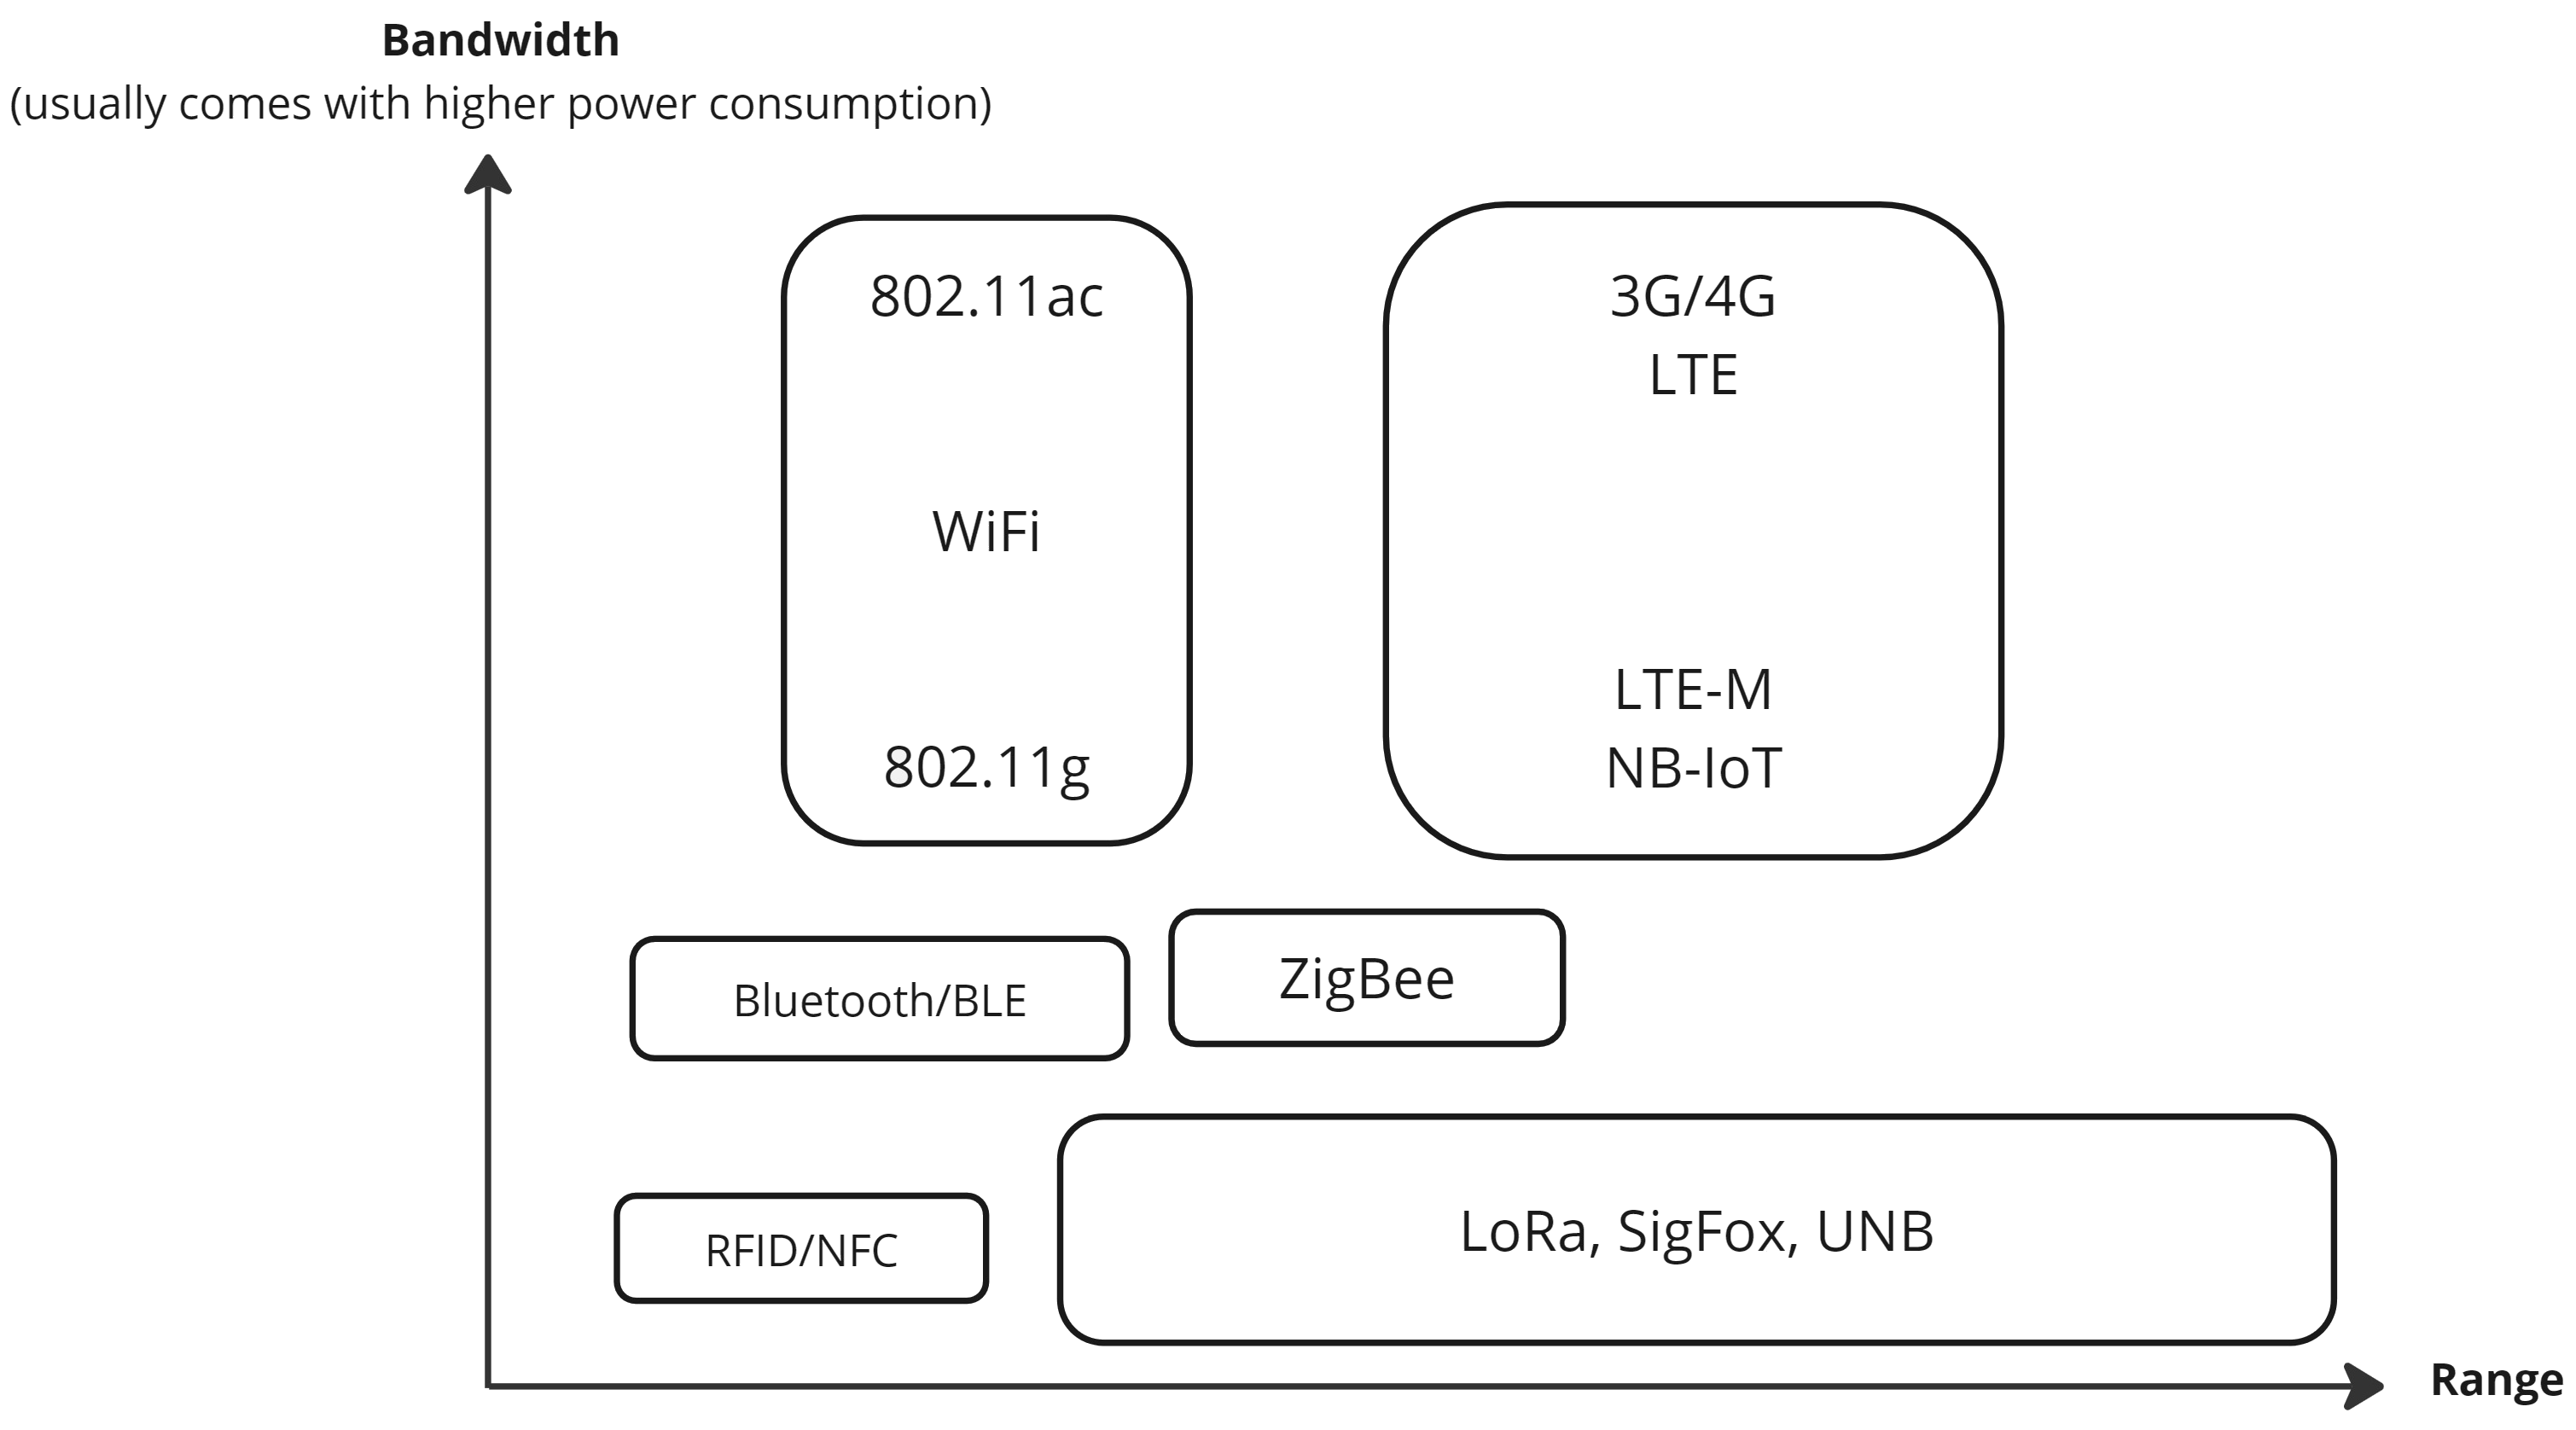
\includegraphics[width=0.8\textwidth]{figures/range_bandwidth.png}
    \caption{Plot showing bandwidth versus the range of different wireless communication technologies. Rework from: \url{https://www3.cs.stonybrook.edu/~mdasari/courses/cse570/lora.pdf}}
    \label{fig:LoRa_bandwidth_range}
\end{figure}

\ac{LoRa} refers to the physical layer and the proprietary spread spectrum modulation technique developed by Semtech. In contrast, \ac{LoRaWAN} refers to the network layer that defines the communication protocol and system architecture, enabling devices to communicate with \ac{LoRa} gateways and network servers. 

\begin{figure}[H]
    \centering
    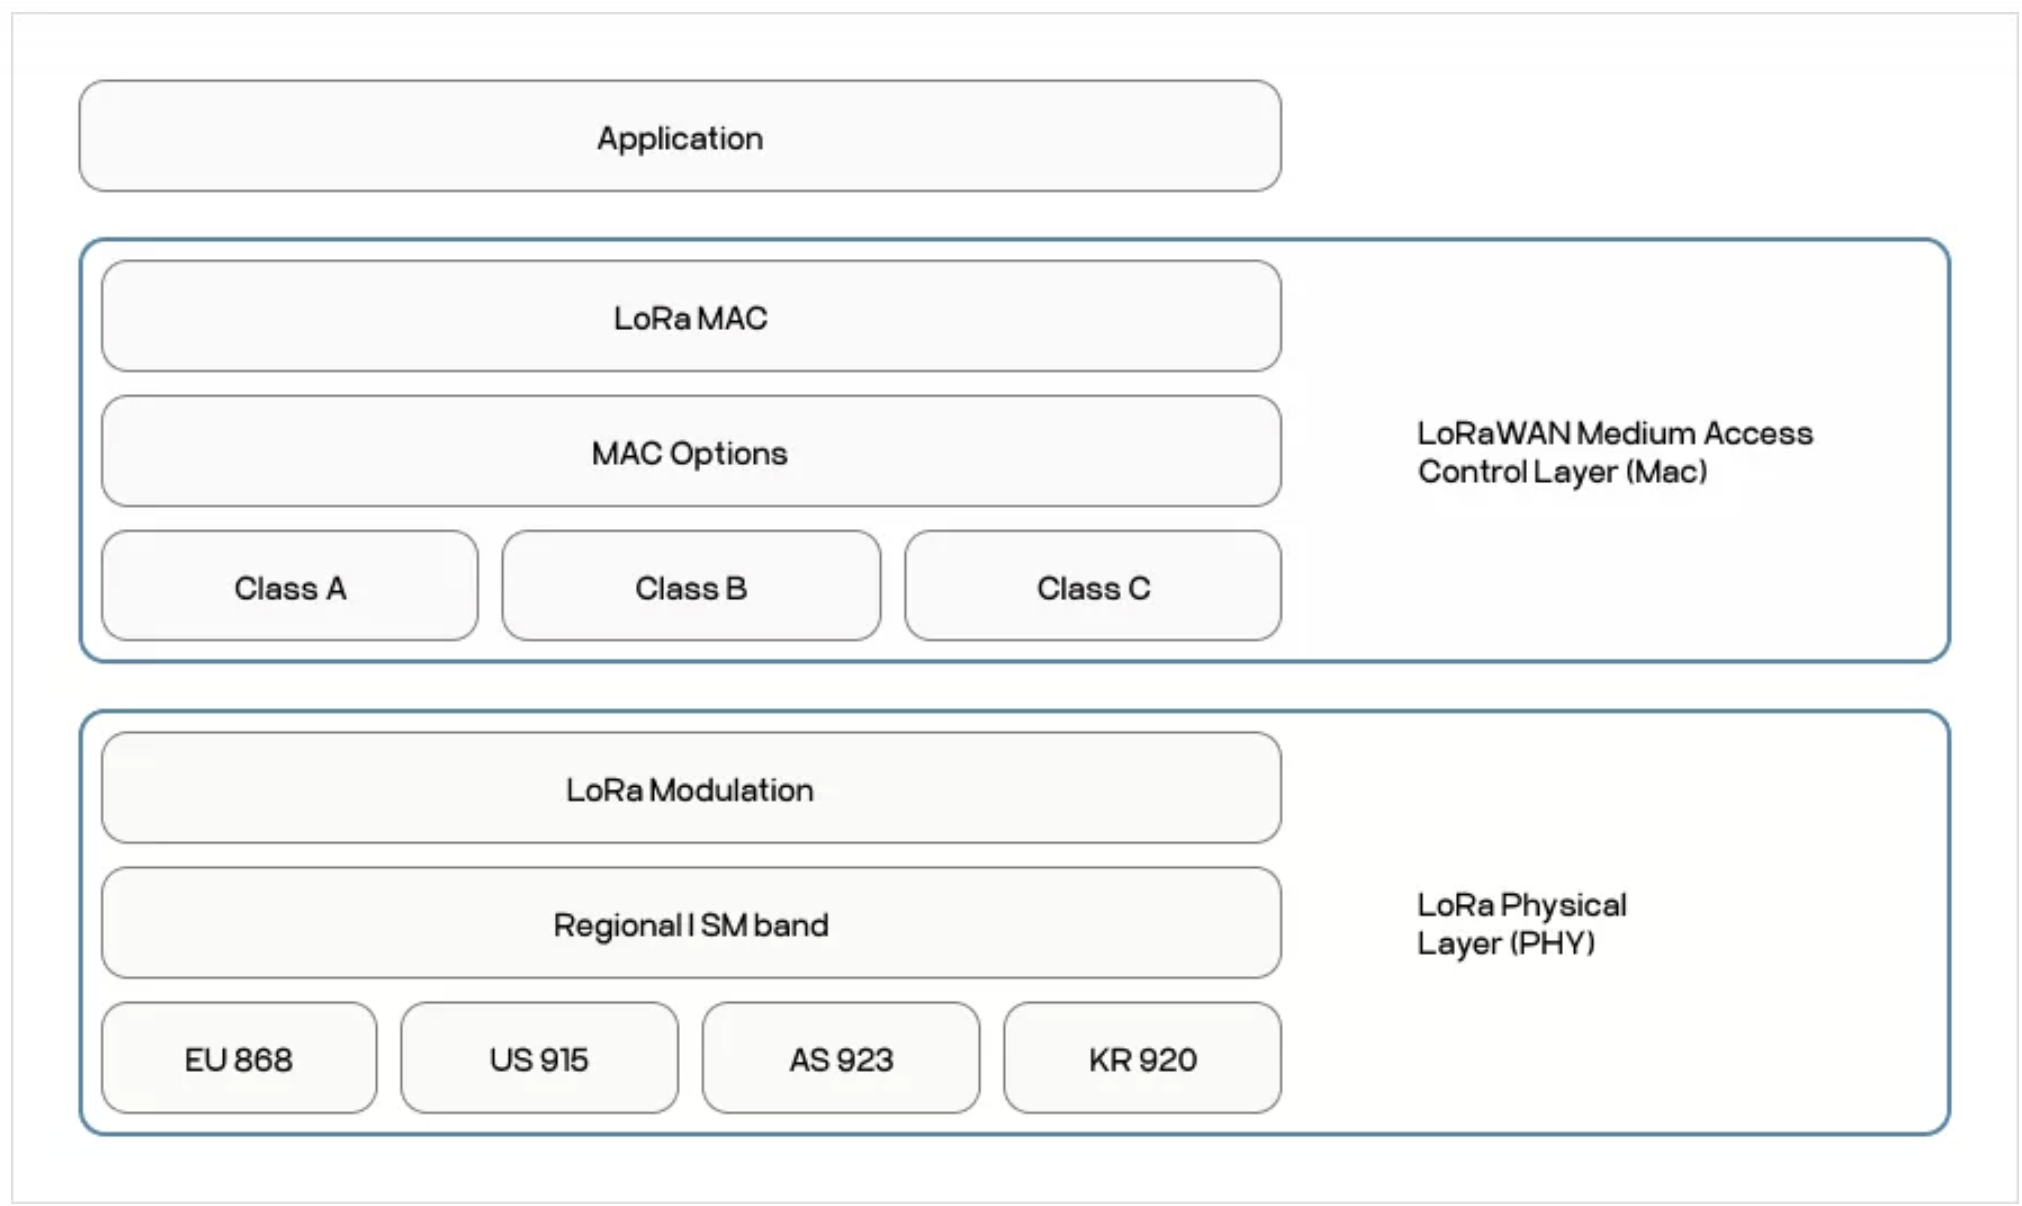
\includegraphics[width=0.8\linewidth]{figures/image.png}
    \caption{\url{https://sirinsoftware.com/blog/lorawan-mac-layer-definition-architecture-classes-and-more}}
    \label{fig:enter-label}
\end{figure}

\subsubsubsection*{LoRa}
LoRa, derived from Chirp Spread Spectrum (CSS) technology, encodes information on radio waves using frequency-modulated chirp pulses, where a chirp is a sinusoidal signal whose frequencies vary linearly over time. When illustrated in the time- and frequency domain, a chirp looks like this:

\begin{figure}[H]
    \centering
    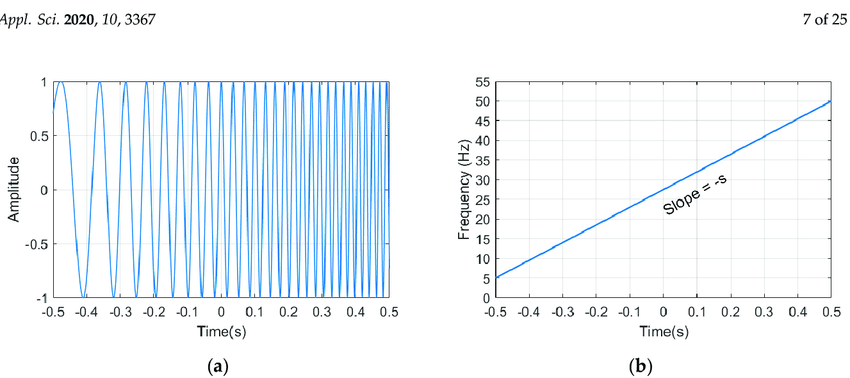
\includegraphics[width=0.9\textwidth]{figures/linear-chirp-up-signal.png}
    \caption{Linear up-chirp signal: (a) Time domain representation. The signal's frequency increases linearly as time passes; (b) The variation of the frequency of the signal that is illustrated in panel (a). Rework from: \url{https://www.researchgate.net/figure/Linear-up-chirp-signal-a-Time-domain-representation-The-signals-frequency-increases_fig4_341373286}}
    \label{fig:LoRa-upchirp}
\end{figure}

(\url{https://en.wikipedia.org/wiki/Chirp_spread_spectrum)}
(\url{https://www.thethingsnetwork.org/docs/lorawan/what-is-lorawan/})

LoRa is the physical layer of the protocol and is responsible for transmitting the raw bit stream over the physical medium.
We want to go into much detail about how the technology works but will stick to describing the major points that influence data rate, power usage and range, which are bandwidth, sweep rate/\ac{SF} and coding factor.

\textbf{Bandwidth (BW):} is the frequency range that the signal sweeps over. Increasing the bandwidth, increases the data rate (decreases \ac{ToA}), but reduces the resistance to noise and interference, and therefore the range. Making the bandwidth 2x wider (from BW125 to BW250) allows you to send 2x more bytes at the same time.
In Europe, the bandwidth is restricted to \SI{125}{\kilo\hertz} and \SI{250}{\kilo\hertz}.

\textbf{Spreading factor (SF):} is a word for how fast the sweep changes over the chosen bandwidth. The quicker the sweep rate, the more information can be passed in a shorter time decreasing the \ac{ToA}, but making the signal more sensitive to noise which reduces the range. Making the \ac{SF} one step lower (from SF10 to SF9) allows you to send 2 times more bytes simultaneously.

\begin{figure}[H]
    \centering
    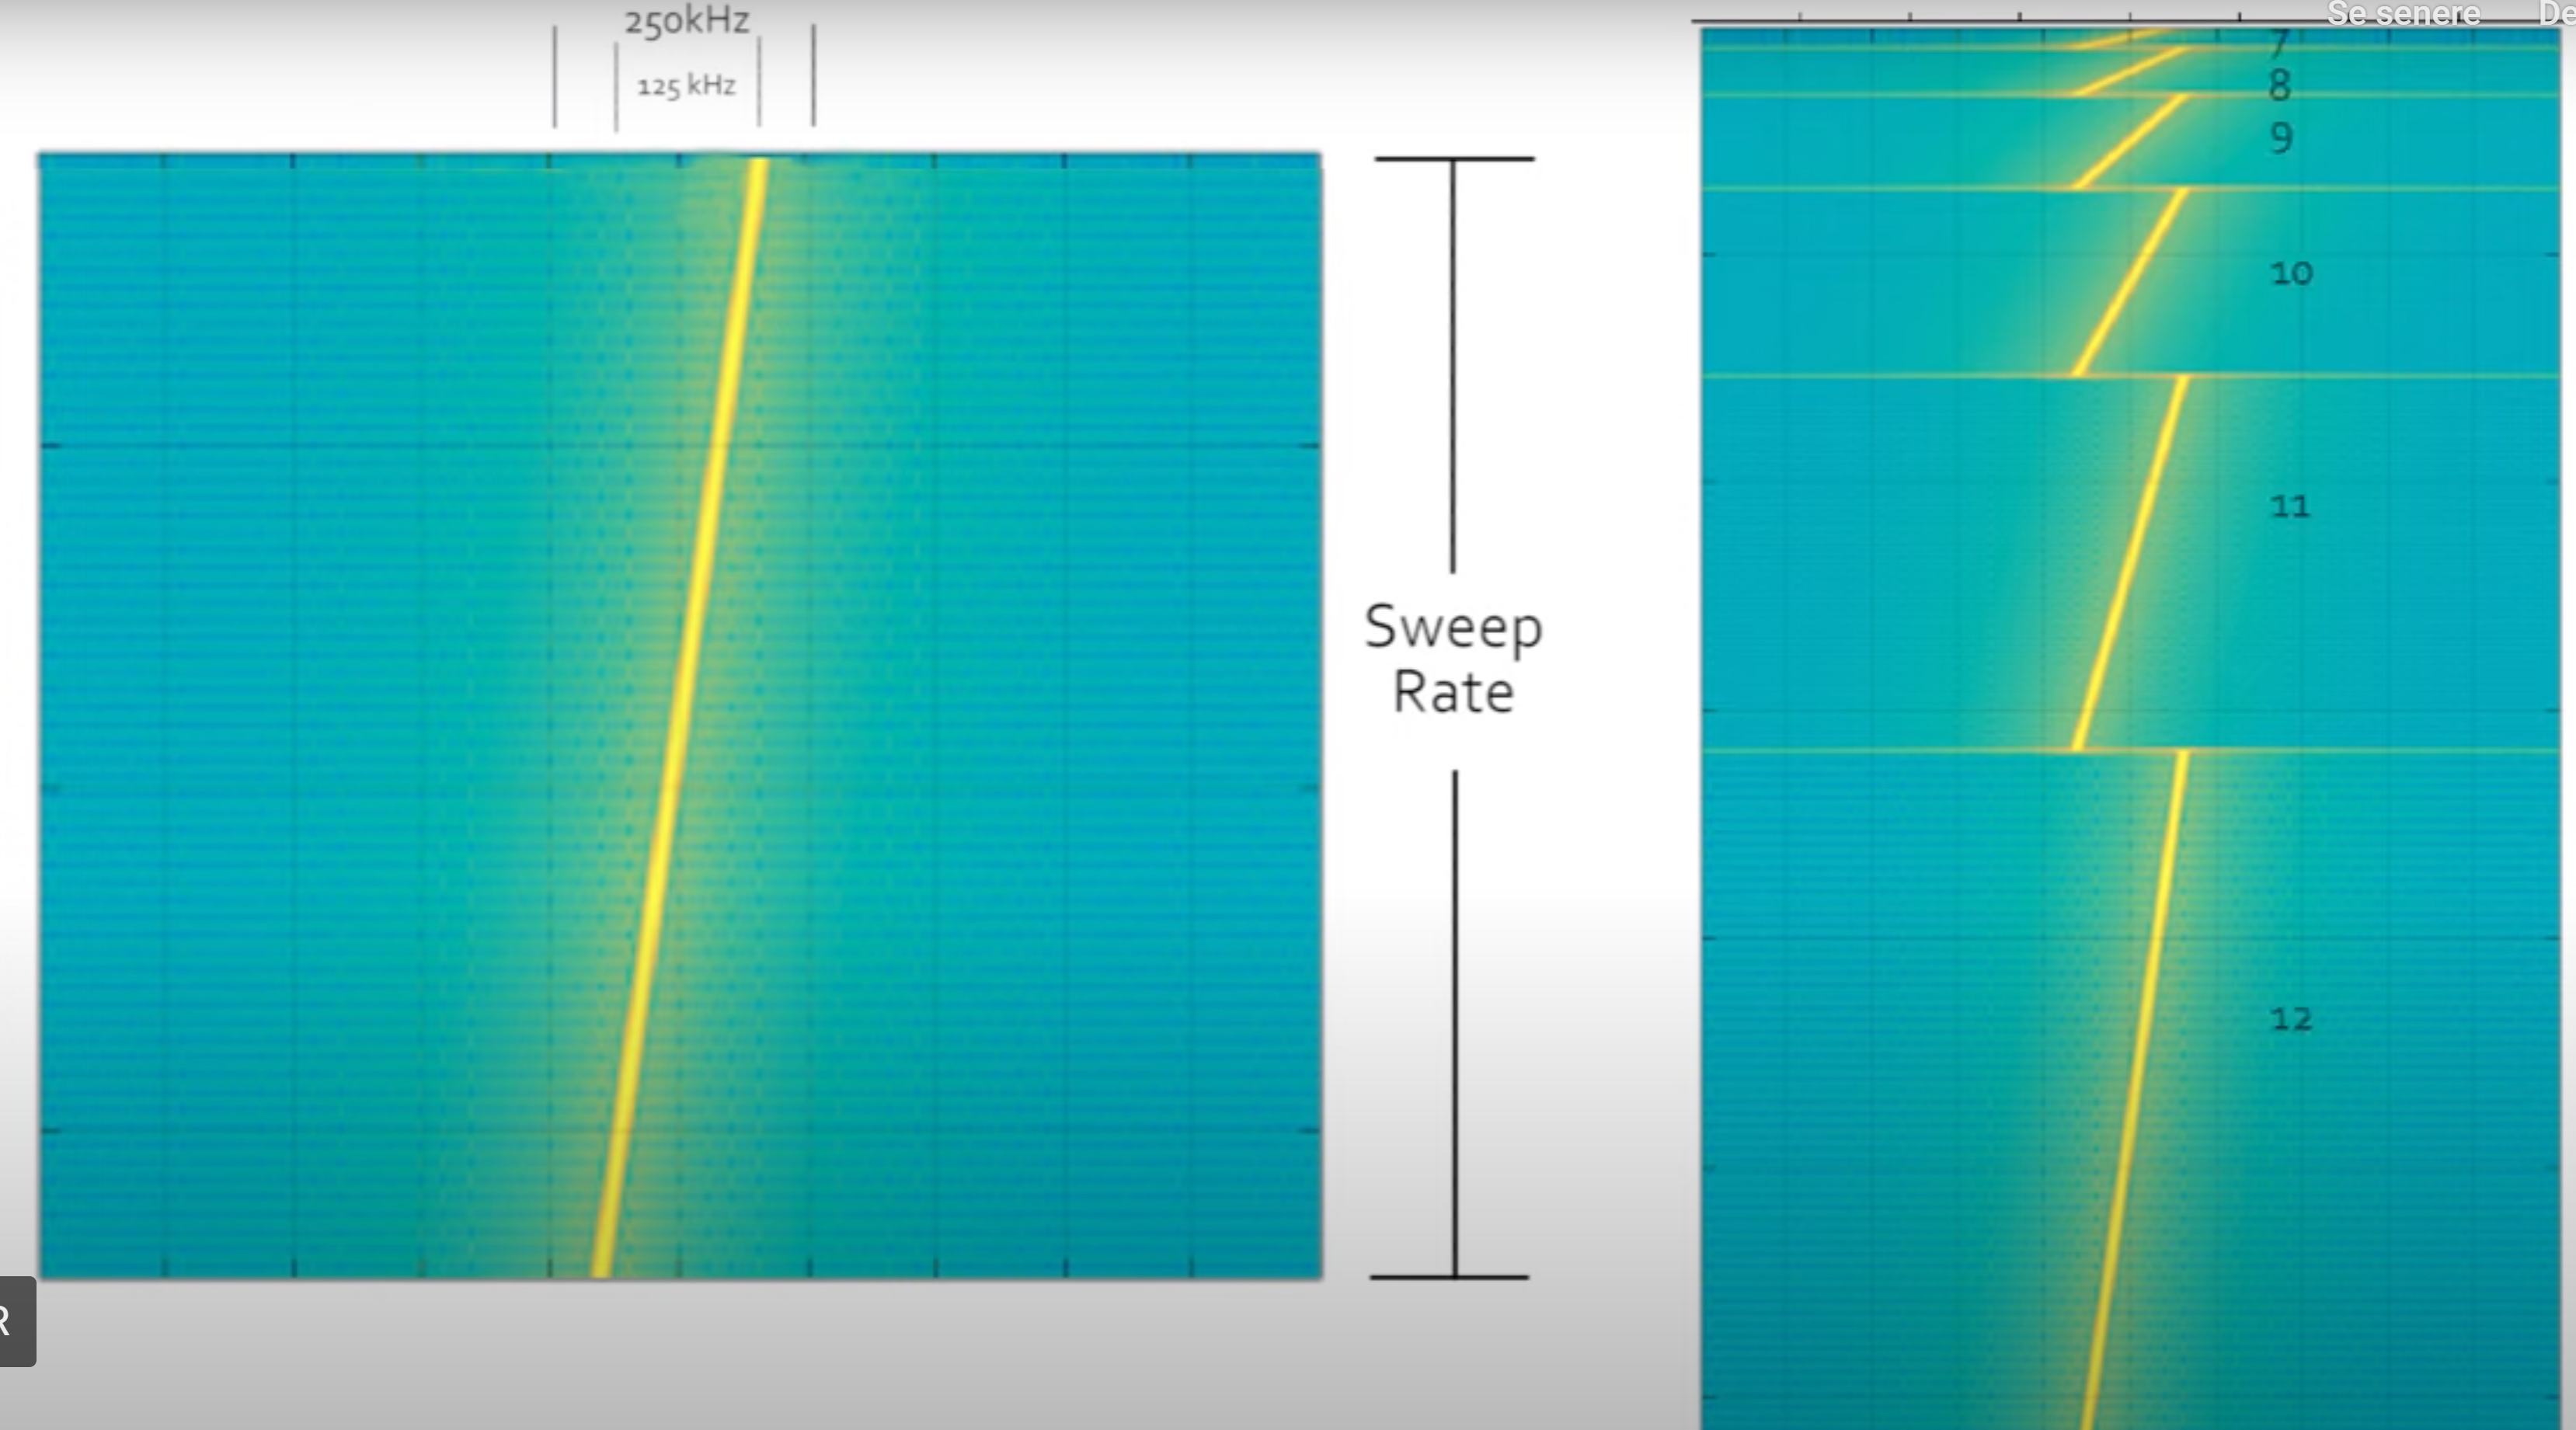
\includegraphics[width=0.8\textwidth]{figures/sweep_rate.png}
    \caption{Spreading factor and more (skal laves selv, eller reference) \url{https://www.thethingsnetwork.org/docs/lorawan/what-is-lorawan/}}
    \label{fig:spread_rate}
\end{figure}

\textbf{The Code Rate (CR):} in \ac{LoRaWAN} determines the number of additional bits added to each payload, which are utilised for error correction purposes. \ac{LoRaWAN} employs four different code rates: 4/5, 4/6, 5/7 and 4/8.
For example, if the code rate is 5/7, for every 5 bits of useful information, 2 extra bits are generated. A higher CR increases the \ac{ToA} but makes communication more robust and therefore also increases the range.

\url{https://iopscience.iop.org/article/10.1088/1742-6596/1407/1/012092/pdf}

\textbf{Time on Air (ToA):} All the above factors influence the package \ac{ToA}, which is a measure of how long it takes to transmit a message. This is the primary factor for battery usage of the end device, as a higher \ac{ToA} results in longer active times for the radio transceivers.

Måske link til den her: \url{https://www.thethingsnetwork.org/airtime-calculator}

All of these parameters can be configured in software, which is the real power of LoRa. As a developer, you can tailor the communication parameters to suit specific requirements, whether prioritising extended transmission distances or minimised power consumption.

\subsubsubsection*{LoRaWAN}
\ac{LoRaWAN} is the \ac{MAC} protocol sublayer on top of the physical (PHY) layer. It is a set of guidelines that dictate how the communication between devices and gateways in a LoRa network should happen. It specifies and handles:
\begin{itemize}
    \item how data should be transmitted; The \ac{MAC} layer structures data into frames for transmission interprets received frames, selects frequency channels for communication and manages the duty cycle, ensuring compliance with regional regulations.
    \item security; The \ac{MAC} layer handles network authentication encryption and decryption, ensuring secure communication between devices and the network.
    \item adaptive data rate; The \ac{MAC} layer dynamically adjusts the data rate based on network conditions, optimising power consumption and communication range.
    \item scheduling and coordination; The \ac{MAC} layer schedules transmissions and manages communication between end devices and gateways, avoiding collisions and optimising network performance.
\end{itemize}

\url{https://sirinsoftware.com/blog/lorawan-mac-layer-definition-architecture-classes-and-more}

\subsubsubsection*{Scheduling: LoRaWAN classes}
\ac{LoRaWAN} supports different classes of devices. These classes define when an end device is allowed to receive downlinks\footnote{end devices can always send uplinks at will}, allowing for intelligent battery and network usage.

Class A: The key characteristic of Class A is that communication is initiated only by the end device. Downlink messages are queued until the end device establishes an uplink. When a connection is established a Class A end device waits a predetermined amount of time (usually one second), and then briefly opens a receive window (Rx1). If no downlink is received within this timeframe, it waits again and proceeds to open a secondary receive window (Rx2). The figure illustrates the different receive window state possibilities for class A. 
This device class is the most energy-efficient and must be supported by an end device.
\url{https://lora-developers.semtech.com/uploads/documents/files/LoRaWAN_Class_A_Devices_In_Depth_Downloadable.pdf}

\begin{figure}[H]
    \centering
    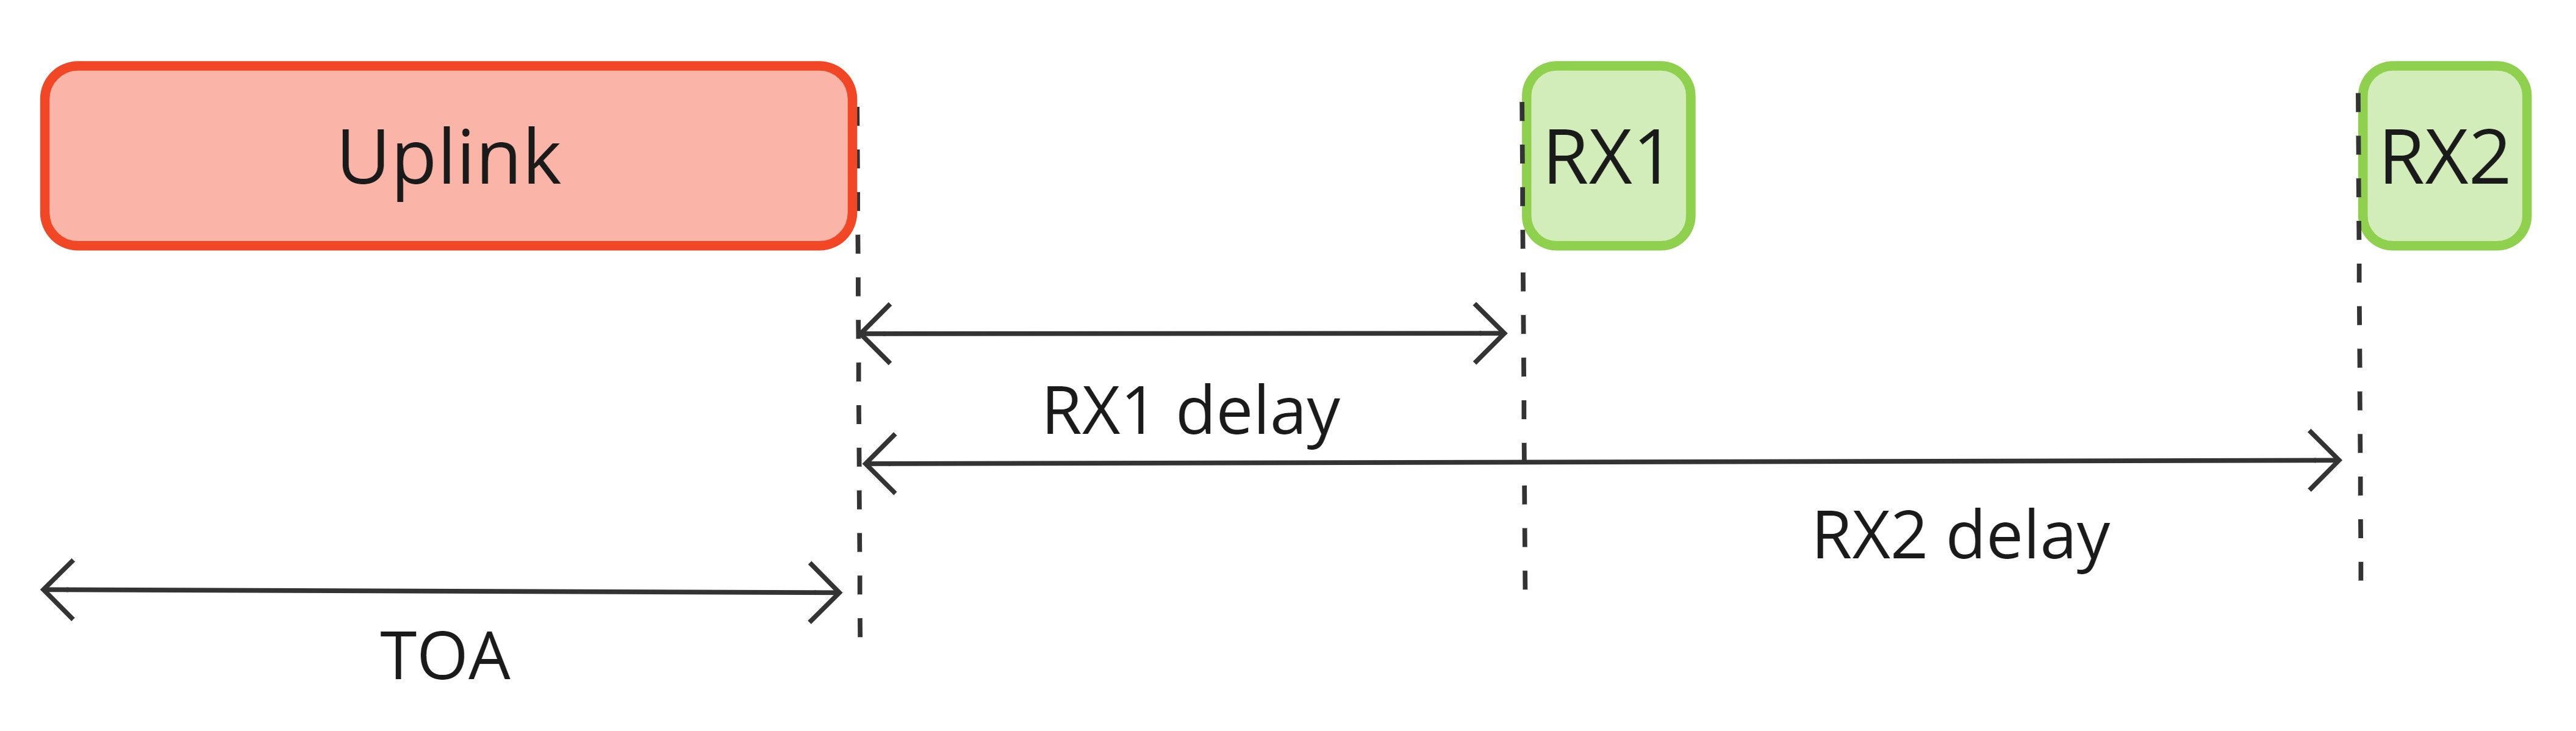
\includegraphics[width=0.7\linewidth]{figures/ClassA_1.jpg}
    \caption{Class A. No received downlink.}
    \label{fig:ClassA-no}
\end{figure}

\begin{figure}[H]
    \centering
    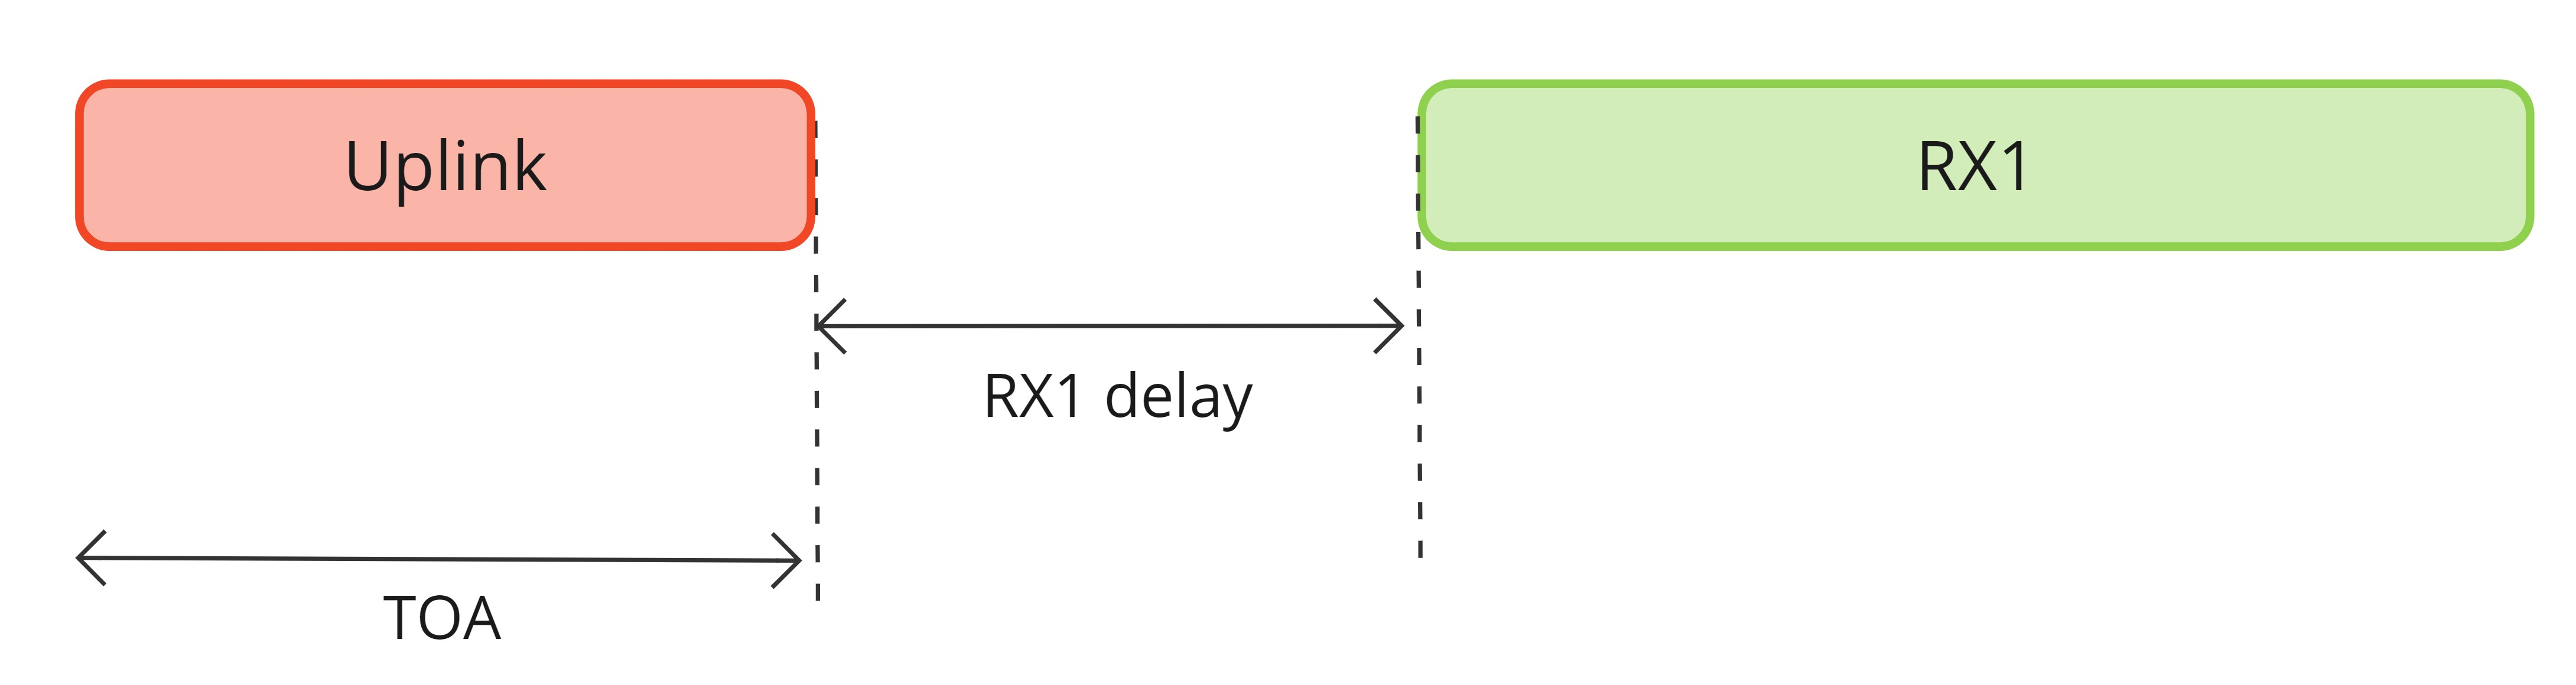
\includegraphics[width=0.7\linewidth]{figures/ClassA_2.jpg}
    \caption{Downlink received in RX1.}
    \label{fig:ClassA-RX1}
\end{figure}

\begin{figure}[H]
    \centering
    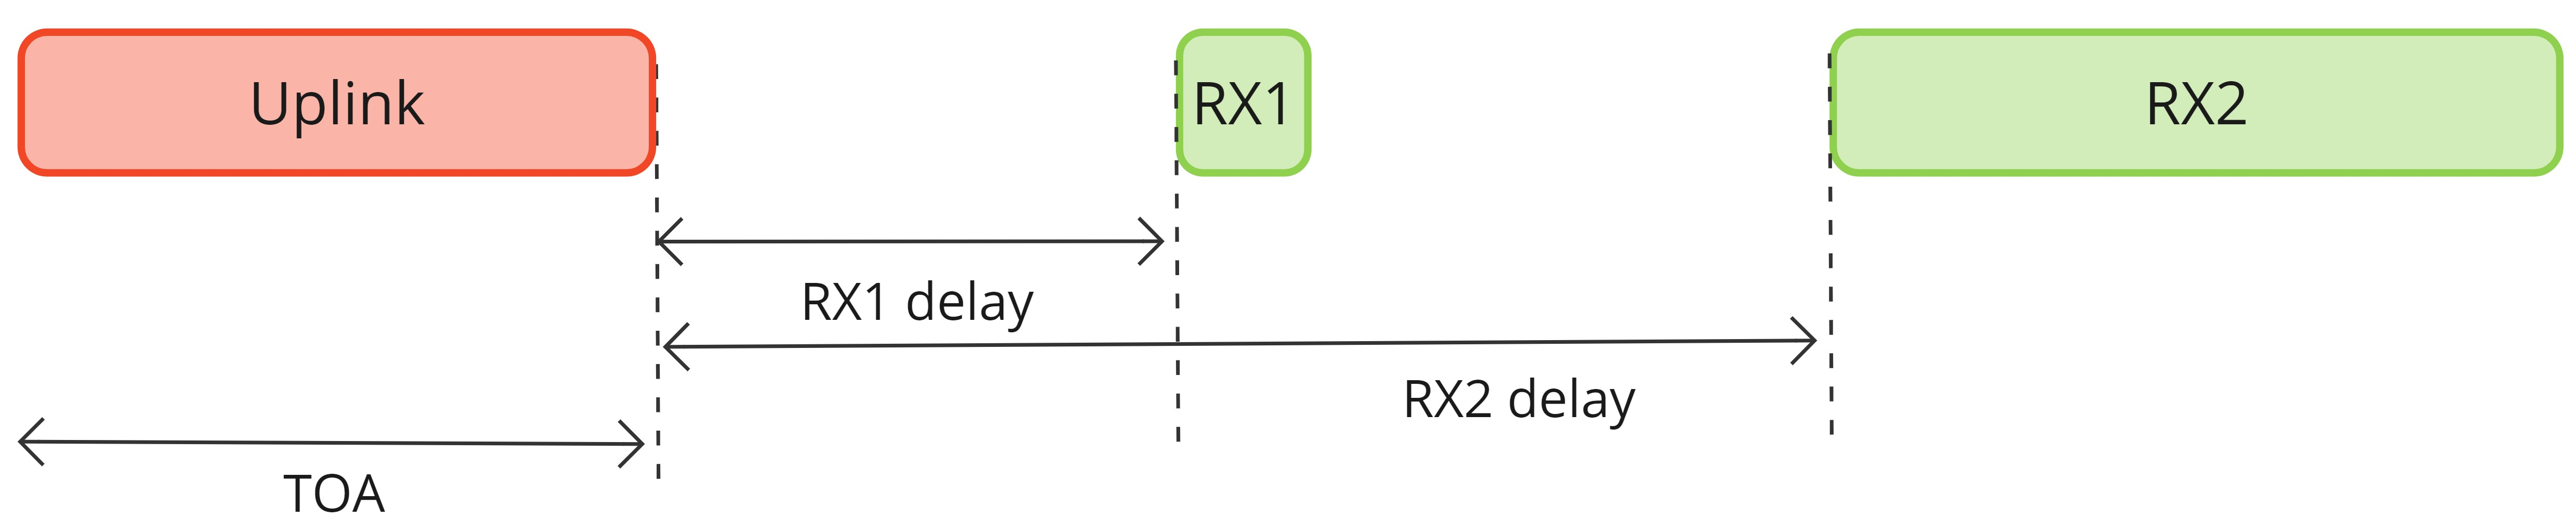
\includegraphics[width=0.7\linewidth]{figures/ClassA_3.jpg}
    \caption{Downlink received in RX2.}
    \label{fig:ClassA-RX2}
\end{figure}

Class B (beaconing): builds on top of Class A, by providing regularly scheduled receive windows, in addition to those that open whenever an uplink is sent.
In class B mode, the end device wakes up after a fixed time interval, ready to receive downlinks. If no downlink is detected, it goes back to sleep. For this to work, the network needs to know when the end device is ready to receive. To do this, a time-synchronized beacon is broadcast periodically by the network via the gateways, to align the end device internal clock with the network.

\begin{figure}[H]
    \centering
    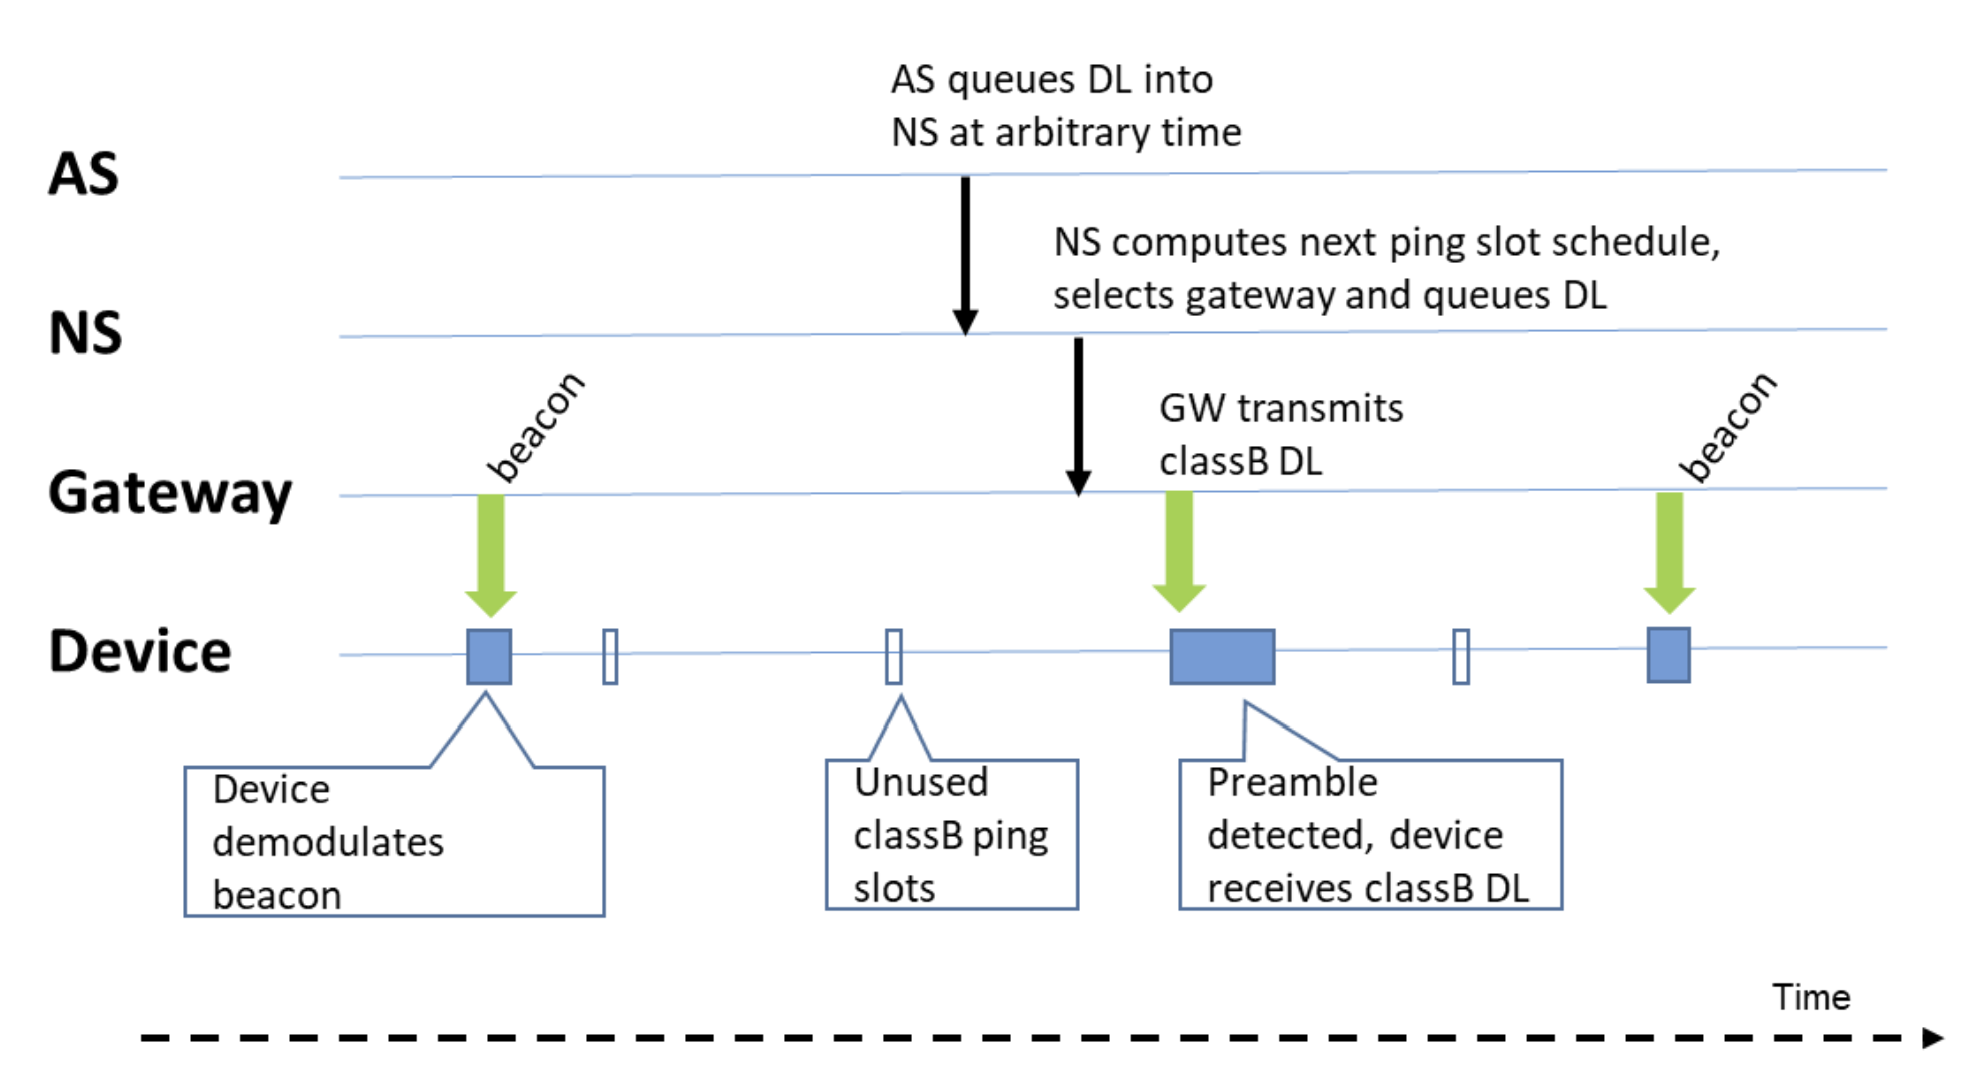
\includegraphics[width=0.7\linewidth]{figures/class_B.png}
    \caption{Class B \url{https://lora-developers.semtech.com/uploads/documents/files/LoRaWAN_Class_B_Devices_In_Depth_Downloadable.pdf}.}
    \label{fig:Class_B}
\end{figure}

Class C (continuous): implements the same schedule as class A with two receive windows, but they do not close the RX2 window until they send the next transmission.

\subsubsubsection*{LoRaWAN Things Stack:}

Gateway server:
manages gateways and creates secure connections with the network server.

The network server: 
implements the \ac{LoRaWAN} protocol
it validates the authenticity and integrity of devices
Deduplicates uplinks
Selects the gateways used for downlinks
Sends ADR commands to optimise the data rate of devices

Hearth of every \ac{LoRaWAN} network/to operate a \ac{LoRaWAN} network you need one.
Main responsibility:
- security
- data routing
- battery optimisation
// All the above of \ac{LoRaWAN} nodes

Application server:
the decryption of the received sensor
encrypts data sent to the device

Join server:
stores the root keys of the devices
Generates session keys to the network server and application server

Identity server:
registers users, applications, devices and gateways

AES-128-based secure low-power communication for \ac{LoRaWAN} IoT environments K tsai

\begin{figure}[H]
    \centering
    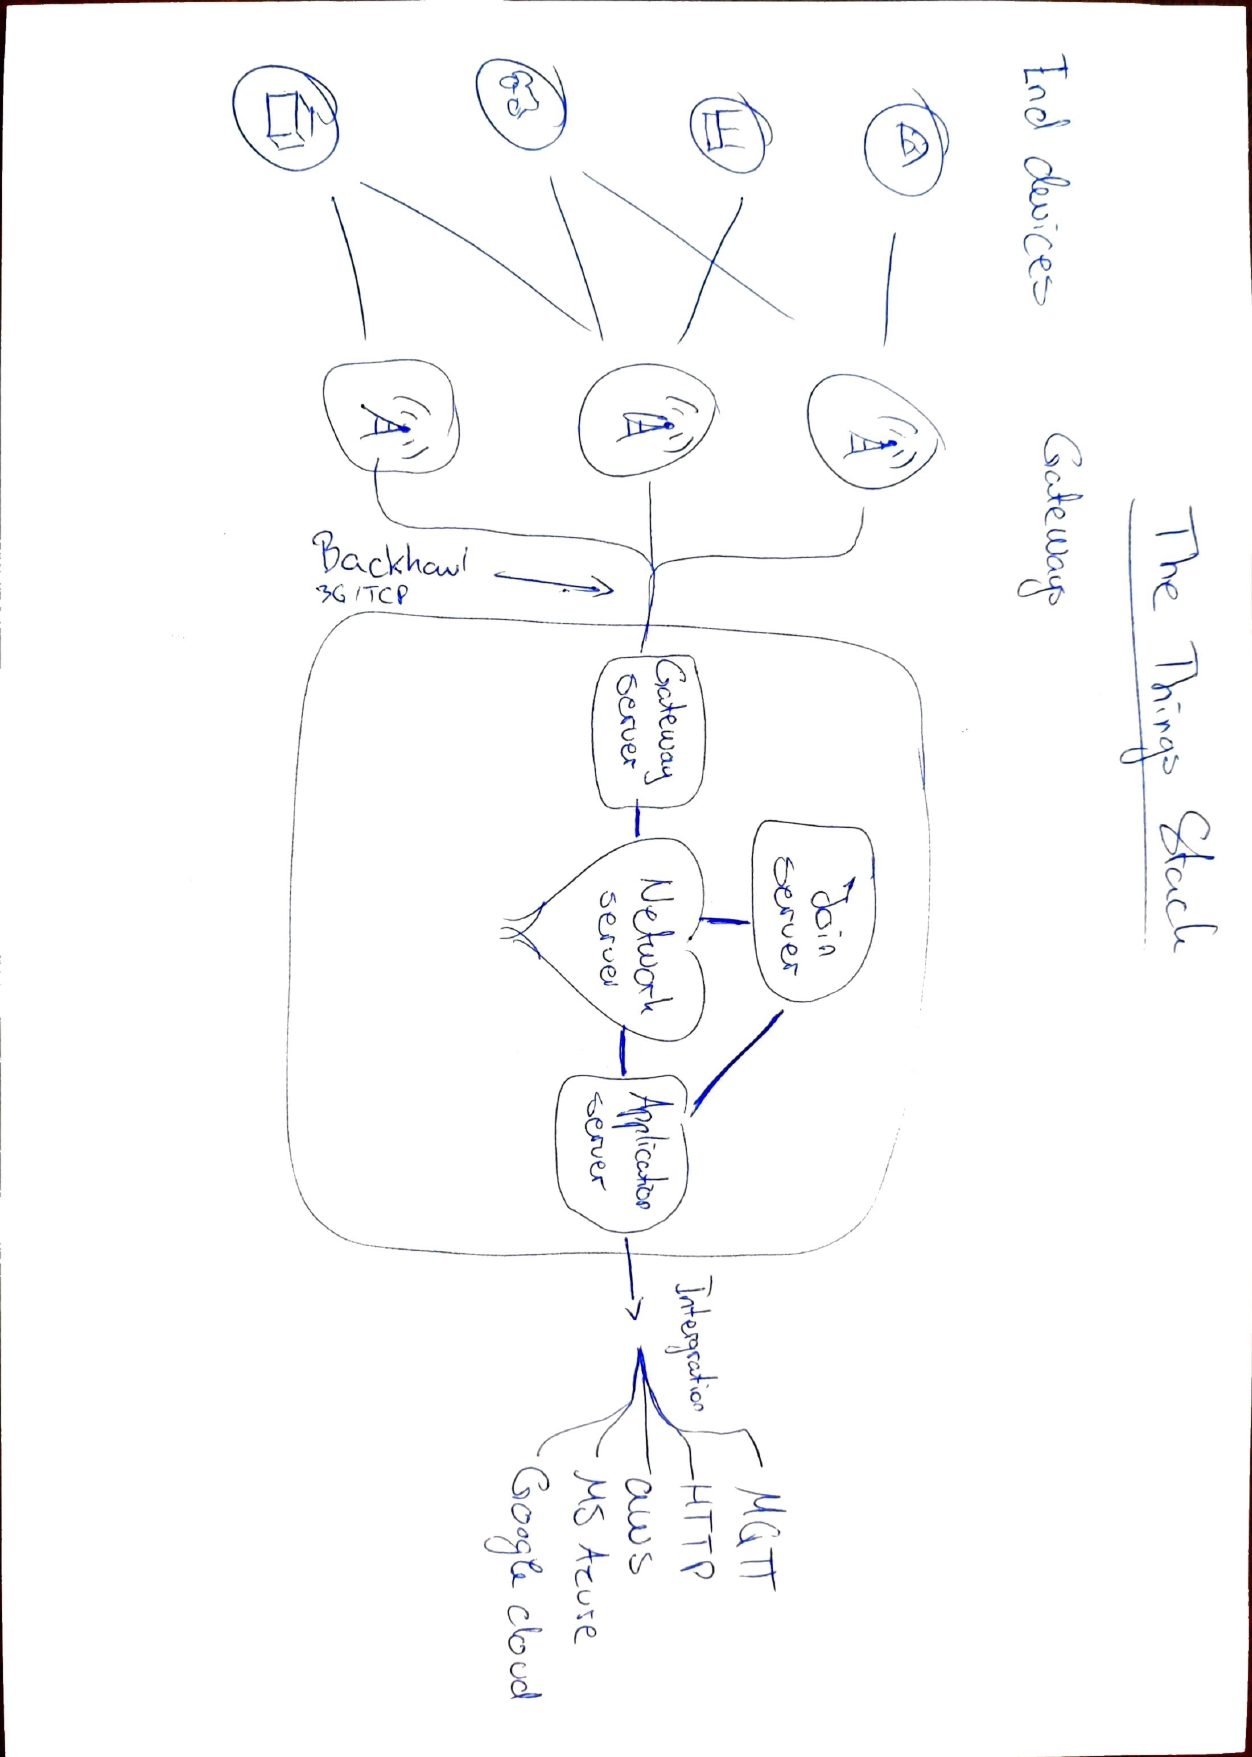
\includegraphics[width=0.8\textwidth]{figures/The Things Stack_page-0001.jpg}
    \caption{setup)}
    \label{fig:LoRaWAN_stack}
\end{figure}
















\ac{DevEUI} (also known as ChipEUI) is like a \ac{MAC} address, a unique identifier for the device. It is a 64-bit number that is assigned to the device by the manufacturer. The \ac{DevEUI} is used to identify the device in the network and is used in the activation process. \ac{JoinEUI} (also known as AppEUI) is a 64-bit number that is used to identify the network server in the activation process. The AppKey is a 128-bit number that is used to encrypt the messages between the device and the network server. The AppKey is used in the activation process to derive the NwkSKey and AppSKey.


%https://www.loracloud.com/documentation/join_service?url=glossary.html#term-Join-Server

Fig.~\ref{fig:LoRa_bandwidth_range} shows the difference between Wi-Fi and \ac{BLE}, versus \ac{LoRa} and cellular signals, comparing the range of the signal travelling and the bandwidth of the signal.

\ac{LoRaWAN} communicates on different frequencies depending on where the device is located; EU: \SI{868}{\mega\hertz} and \SI{433}{\mega\hertz}, US: \SI{915}{\mega\hertz}, AS: \SI{430}{\mega\hertz}.

SKRIV OGSÅ OM PRIS OG GATEWAYS PÅ LORAWAN
Evt.indsæt billede af Topology. End nodes <-> Gateways (private or corporate) <-> Network server <-> Application server

\ac{SF}

\subsubsection{HTTP/REST API}
Måske vil skal skrive noget om dette

\subsection{The LoRaCloud ecosystem}
Join server
Modem \& geolocation services

\begin{figure}[H]
    \centering
    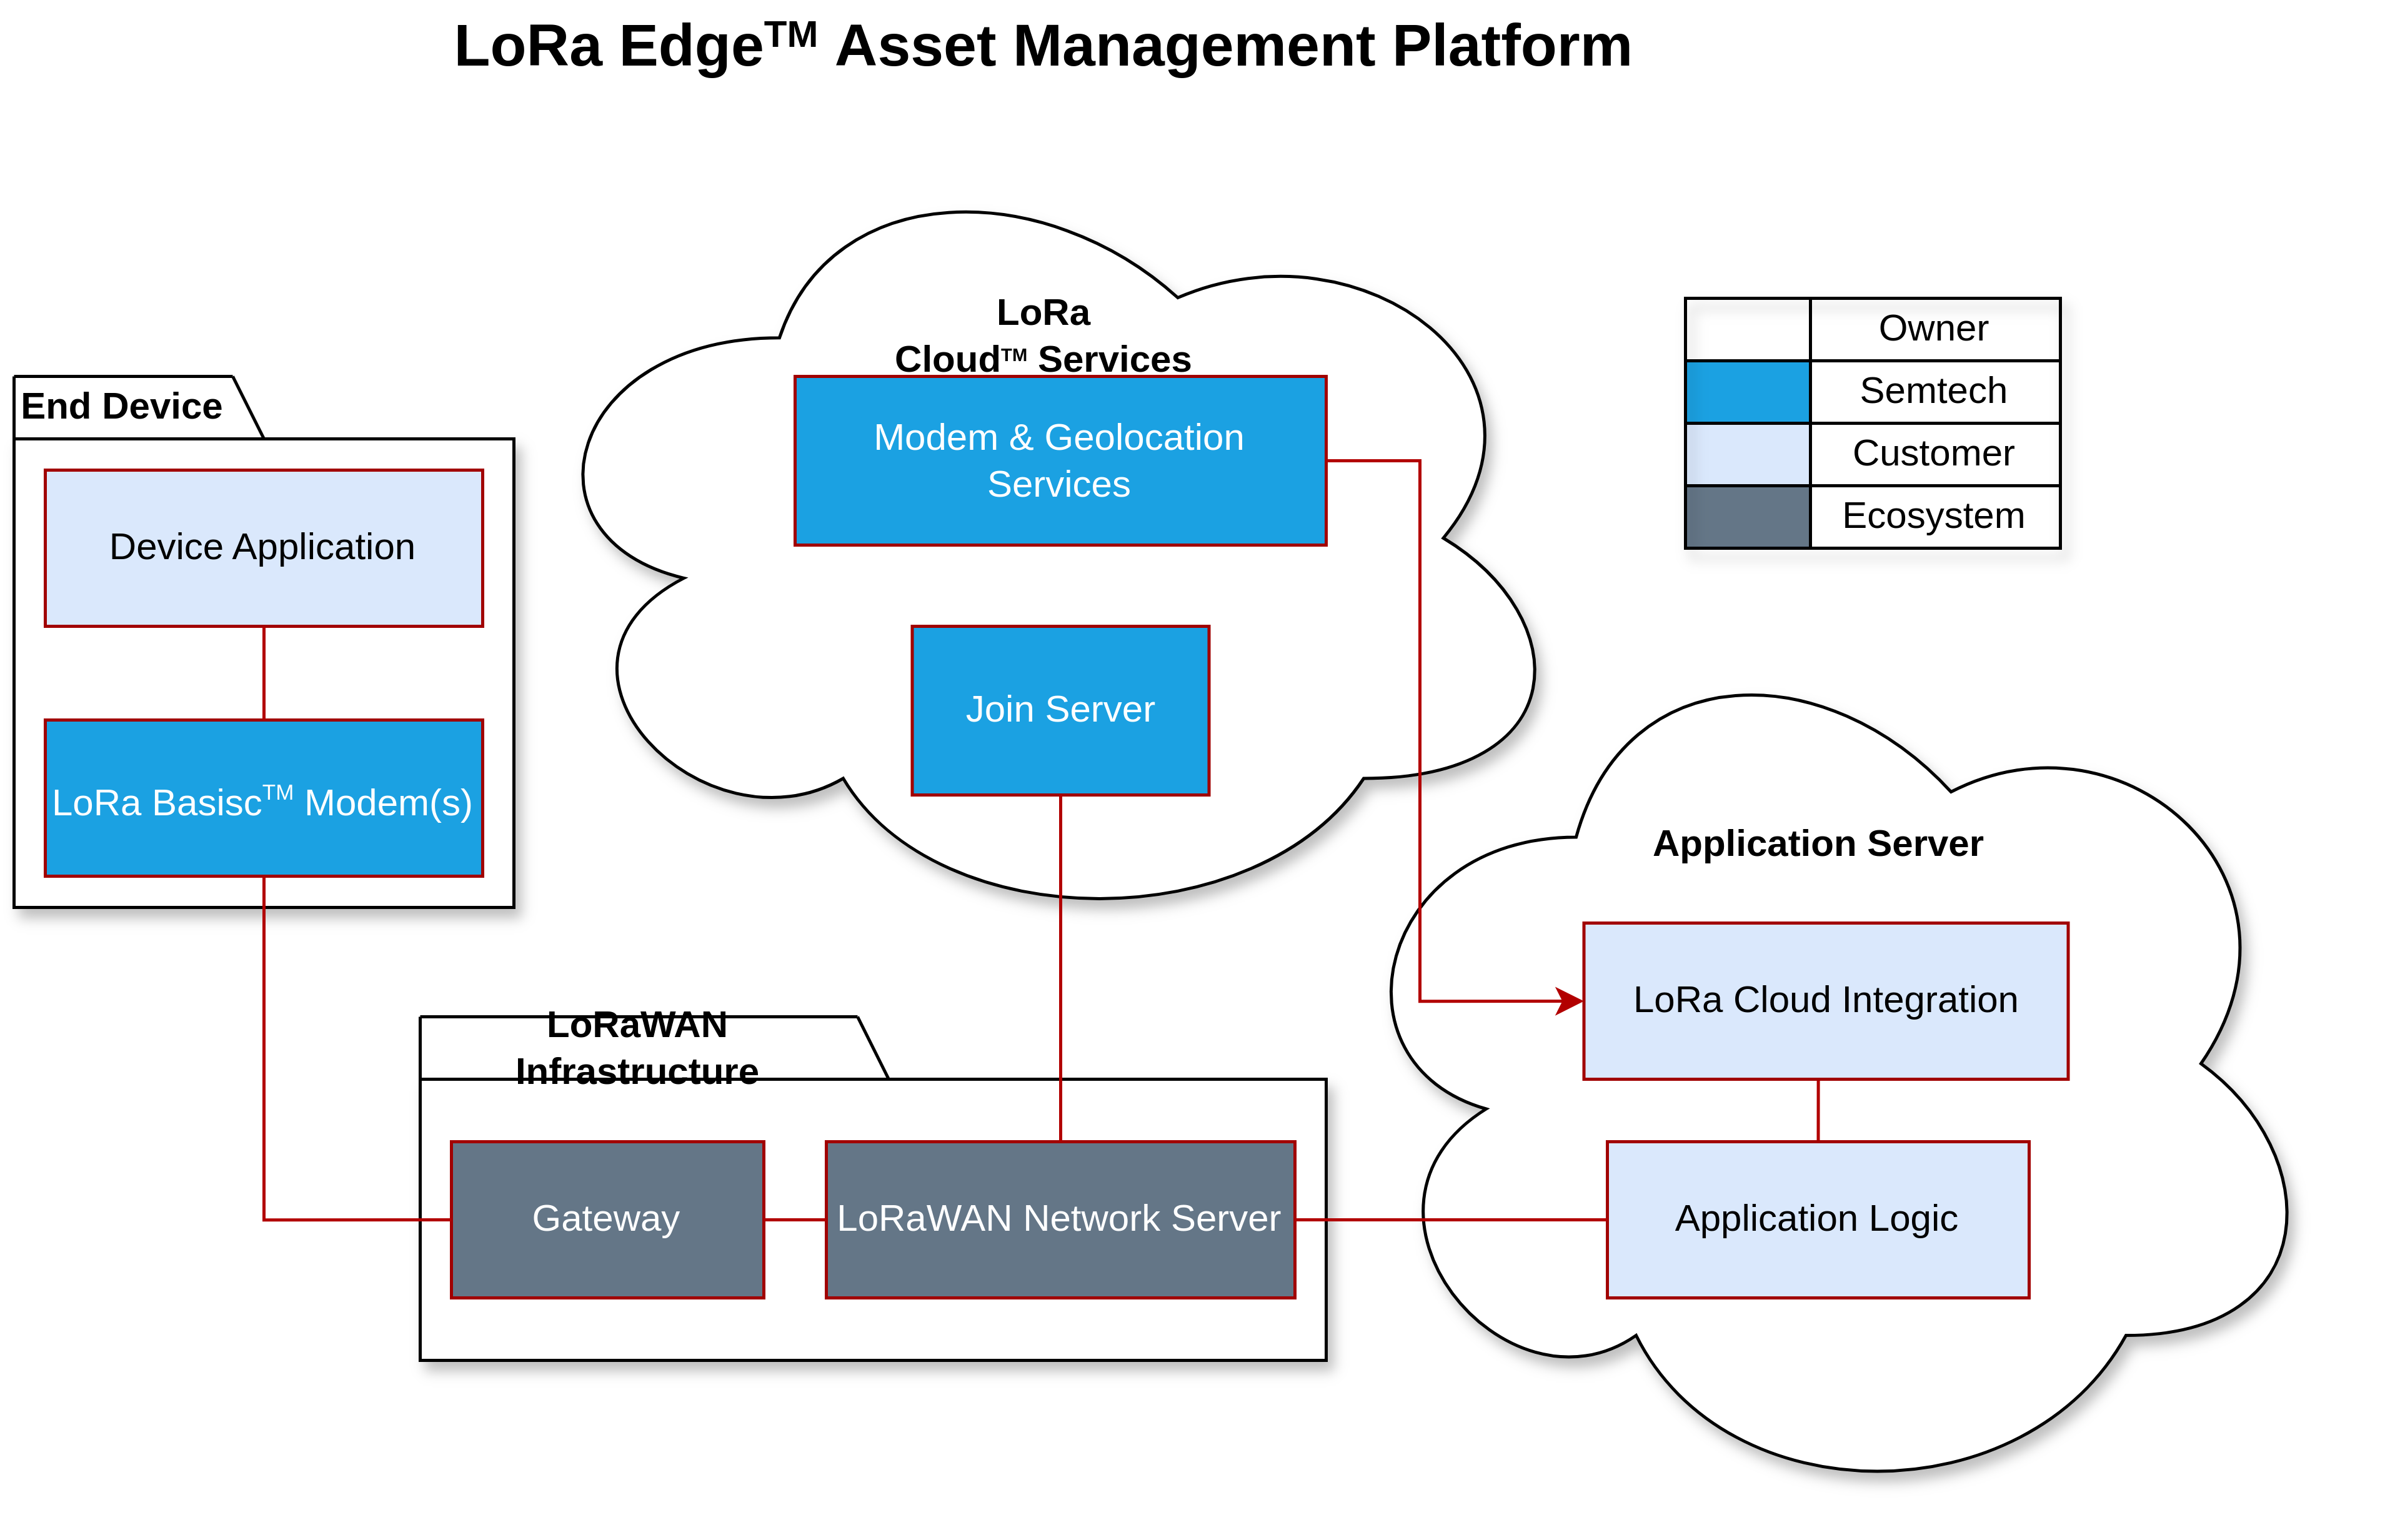
\includegraphics[width=0.7\linewidth]{figures/LoRaCloud_interface.png}
    \caption{LoRa Edge\textsuperscript{\texttrademark} Asset Management Platform}
\end{figure}

\subsection{Geopositioning}
Geopositioning or geolocation is the process of determining or estimating the geographic position of an object \cite{ISO19130}. This can be done using many different methods, each with strengths and weaknesses regarding workload and accuracy. This thesis focuses on using Wi-Fi and \ac{GNSS} combined with Google\footnote{Google Geolocation API: \hangindent=2em \url{https://developers.google.com/maps/documentation/geolocation/overview}} and Semtechs Geolocation APIs \footnote{LoRa Cloud: \url{https://www.loracloud.com/}} to get a general location of the LR1110 chip.

%https://lora-developers.semtech.com/learn/hands-on-labs/build-end-to-end-solution-using-lorawan-and-loraedge/find-the-location-of-your-tracking-device/


"Google's Geolocation API is a service provided by Google that allows developers to retrieve the approximate geographical location of a device based on various factors, without necessarily relying on \ac{GPS}. Here's a basic overview of how it works:

\textbf{Request Submission}: The client (a web browser or a mobile app) sends a request to the Geolocation API endpoint with data about nearby Wi-Fi access points, cellular towers, or Bluetooth beacons that the device can detect. This data includes information like the \ac{MAC} addresses of Wi-Fi access points, cell tower IDs, signal strengths, and other relevant parameters.

\textbf{Data Processing}: Google's servers receive the request and analyse the data provided. They compare the received data against a vast database of known Wi-Fi access points, cell tower locations, and their corresponding geographical coordinates. Google continuously collects this data through its Street View cars, mobile mapping vans, and other sources, building a massive database of Wi-Fi and cell tower locations worldwide.

\textbf{Triangulation and Trilateration}: Using the information gathered from nearby Wi-Fi access points, cellular towers, and other available signals, Google's servers apply techniques like triangulation and trilateration to estimate the device's location. Triangulation involves determining the device's position by measuring the angles between it and known points (e.g., Wi-Fi access points). Trilateration involves calculating the device's position based on its distance from multiple known points.

\textbf{Response}: After processing the request and estimating the device's location, the Geolocation API returns a response containing the latitude and longitude coordinates of the device's approximate location. Additionally, the response may include other information such as the accuracy of the location estimate and a confidence radius.

\textbf{Privacy Considerations}: Google implements measures to protect user privacy when using the Geolocation API. For example, the \ac{API} may not return precise location data in certain cases, and users have control over their location-sharing settings through their device settings and Google account preferences.

Overall, Google's Geolocation API provides a convenient and efficient way for developers to determine the approximate geographical location of a device without relying solely on \ac{GPS}, making it useful for a wide range of location-based applications and services."

%https://samy.pl/mapxss/
%https://developers.google.com/maps/documentation/geolocation/overview
%https://blog.invgate.com/how-to-locate-a-device-using-a-mac-address
%https://blog.semtech.com/indoor-wi-fi-geolocation-with-lora-edge
%https://lora-developers.semtech.com/community/faq/faq-geo-location
%https://lora-developers.semtech.com/learn/hands-on-labs/build-end-to-end-solution-using-lorawan-and-loraedge/find-the-location-of-your-tracking-device/

\subsubsection{GNSS positioning}

The LR1110 features a fast and low-power \ac{GNSS} scanner. The device captures a short portion of the signal broadcast by the
\ac{GNSS} satellites and extracts the information required to calculate the device position - the pseudo ranges. This information is aggregated into a \ac{NAV} which can be sent to a solver to compute the device position.

\begin{figure}[H]
    \centering
    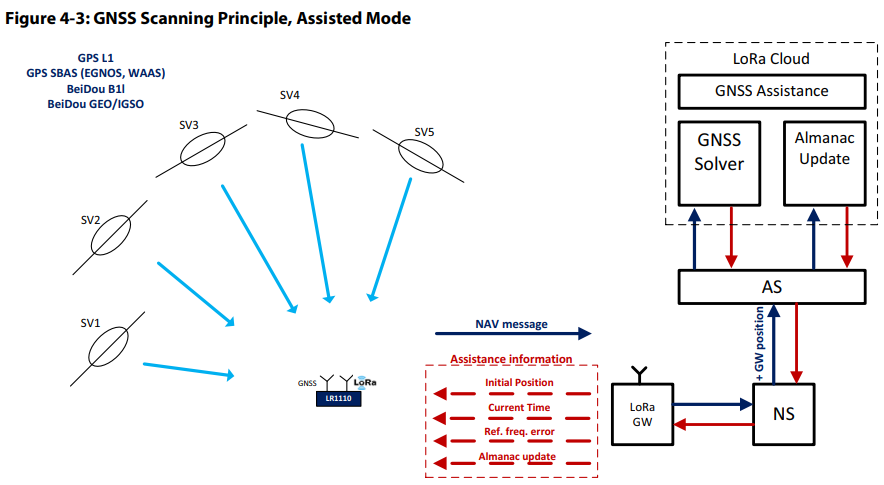
\includegraphics[width=0.9\textwidth]{figures/GNSS_scanning.png}
    \caption{GNSS Scanning Principle, Assisted Mode.}
    \label{fig:gnss_scanning}
\end{figure}
% taken from: https://semtech.my.salesforce.com/sfc/p/#E0000000JelG/a/3n000000vBus/cPXIY7jwqFWpmW7USMtfqpJt7T5afR439wbYefi4tsI page 17

Providing assistance information to the LR1110 will minimize the search space, reducing the capture time and the energy spent.

The \ac{GNSS} scanner of the LR1110 has two modes of operation: autonomous and assisted.

\subsubsubsection{Autonomous GNSS Scanning}
The LR1110 will not require any assistance information in this mode. A fast search of all \ac{SV}s with strong signals in the
selected constellation is performed, and all the \ac{SV}s received with a signal better than RXSGPS1E\footnote{RXSGPS1E: GPS, indoor classification, and strong signal \ac{SV} capture. Typ. \SI{-134}{\dB}\cite{LR1110_datasheet}} are detected.
This mode can be used to determine if the device stands indoors or outdoors; in case no \ac{SV} with a strong signal is detected, the application concludes that the device is indoors. Therefore the search for weak signals, which takes more time and energy, can be discarded; the search for other signals of opportunity, like Wi-Fi, might be launched instead.

\subsubsubsection{Assisted GNSS Scanning}
Based on the assistance information, the LR1110 will build a list of 10 to 12 \ac{SV}s that it should look for at the position of the device and the actual time.
Two different assisted \ac{GNSS} scanning modes are implemented:
\begin{itemize}
\item \textbf{Low power}: A first search of strong signal satellites within the list of visible ones will be made. If at least one satellite is found in this step, the search will continue for satellites with weaker signals. Otherwise, the search will stop. This mode minimises energy consumption and can also be used as an indoor/ outdoor detection method, in a more efficient way than the autonomous \ac{GNSS} scanning mode. The indoor classification is decided after searching 10-12 \ac{SV}s, versus 32-35 in Autonomous scanning mode.
\item \textbf{Best effort}: A first search of \ac{SV}s with strong signals, within the list of visible satellites, is made. Even if no satellite is found in the first phase, the search continues for satellites with weaker signals. This mode is to be used in difficult environments where it may be possible to find \ac{SV}s, at the expense of a longer search phase.
\end{itemize}
The scanner uses a sequence of capture and processing phases. To reserve power, the \ac{RF} front end will be turned off during the processing phases.

\subsubsection{Wi-Fi positioning/Geolocation databases/API}
Semtech
Google
Apple, Qualcomm, Wiggle

\subsection{Product design}
A brief introduction to what product design is. Maybe how it has changed?

\subsubsection{Prototyping}




3D-printing
However, since interactive systems are complex, it may be difficult or impossible to create prototypes of a whole design in the formative stages of a project.
Choosing the right kind of more focused prototype to build is an art in itself, and communicating its limited purposes to its various audiences is a critical aspect of its use

This chapter aims to establish a model that describes any prototype in terms of the artifact being designed, rather than the prototype's incidental attributes. By focusing on the purpose of the prototype—that is, on what it prototypes

Prototypes provide the means for examining design problems and evaluating solutions. Selecting the focus of a prototype is the art of identifying the most important open design questions

Teksten ovenfra er fra Houde - What do Prototypes prototype?
Skriv om, hvordan prototyper kan teste forskellige ting, og hvordan opmærksomhed på dette inden, kan hjælpe med at få det rigtige udkom af ens prototype.

\subsubsection{Actor-oriented design}
Hvad er en fælles nævner for de forskellige etnografiske feltstudiemetoder?
Det er kvalitativ metode eftersom at dette er essentielt for design, da vi er interesserede i detaljer!

Hvad er induktiv tilgang?
Empirisk induktiv. Man starter med kvalitativ dataindsamling, man finder heraf en induktiv slutning og ser heraf en sammenhæng eller et mønster.
Fx. I et givet tidsrum på et bestemt sted er alle fugle sorte, og man konkluderer heraf at alle fugle er sorte

Hvad er Grounded Theory, samt hvilken tilgang?
Induktiv. En design-ingeniørs måde hvorpå at være undersøgende og starte fra bunden -> vi starter i empirien.
Problemet defineres på baggrund af den data der indsamles. En analyse kan vise mønstre af tematikker.

Hvad hører sammen med kvalitativ data?
Induktiv! Videnskabelig metode som ikke er målbar.

Interviews - Etnografisk felstudie
Hvad er en fælles nævner for de forskellige etnografiske feltstudiemetoder?
Det er kvalitativ metode eftersom at dette er essentielt for design, da vi er interesserede i detaljer!

Hvilken tilgang skal vi helst bruge som design-ingeniører? - Induktiv

Hvad er et etnografisk interview?
Det er en kvalitativ metode.
Et åbent interview hvor man kommer tættere på aktørens kultur og praksis.
Man gør sig fremmed for det felt man undersøger.
Iterativt -> kræver en analyse som ofte leder op til et nyt feltbesøg.

Hvad skal man have med når man forbereder sig til interviews?
Hvilken viden mangler vi?
Hvem ligger inde med den?
Hvem tager vi kontakt til? Hvordan tager vi kontakten?
Hvem faciliterer interviewet?
Hvordan dokumenterer vi undervejs?
Hvor udfører vi interviewet? (on location eller ....?)
Hvordan deler vi viden efterfølgende (optager vi samtalen, skriver vi noter, laver vi arbejdsblade?)

Hvad er et affinitetsdiagram, overordnet?
At gruppere viden (KJ-metoden)
Deling af viden i teamet, fra forskellige kilder.
Fortolkning af viden, analyse.

Skriv ting på post-its og grupper efterfølgende i overordnede temaer.

Hvad tager affinitetsdiagrammer udgangspunkt i?
Grounded theory; derfor, lad empirien tale -vundgå prædefinerede kategorier.
Start med statements/findings og IKKE med overskrifterne.

\subsubsection{Design criteria}
How to set up design criteria.
Here, we must talk about requirements, criteria and wishes.
Requirements are things that must be
Criteria are measurable. This means that they can be more or less fulfilled.
Wishes are nice to have

\subsubsection{Use cases}
How do you find use cases? What are use cases?

\subsubsection{Affinity diagram/KJ-method}
Affinity: a similarity of characteristics suggesting a relationship, especially a resemblance in structures and thoughts.
Affinity mapping gives designers a visual view of their research, capturing data so that themes, trends, and needs emerge.
Affinity mapping is done during the divergent research phase. In this diagram of the Double Diamond, where the first diamond to the left represents research discovery and analysis, affinity mapping can be done multiple times to organise and analyse research data. At the beginning of the design phase, represented by the second diamond on the right, research should be finalised. It is not recommended to do affinity mapping during the design phase.